\documentclass{standalone}
\usepackage{tikz}
\usetikzlibrary{patterns, positioning}


\begin{document}
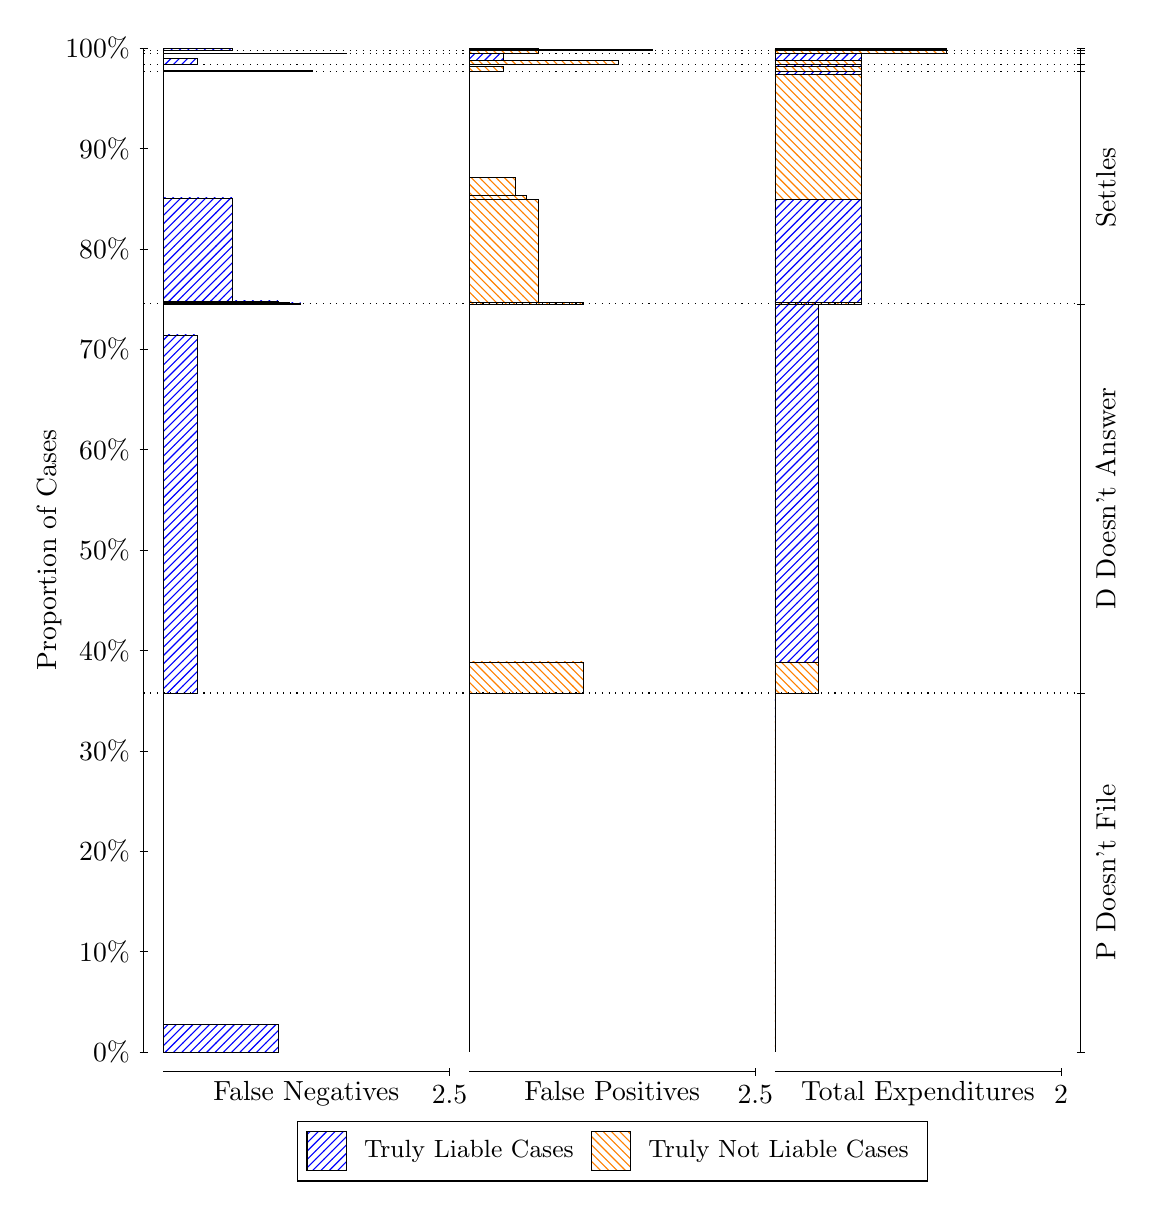
\begin{tikzpicture}
\draw[black, very thin] (1.5,1.75) -- (1.5,14.5);
\node[rotate=90, text=black, anchor=center] at (0.3, 8.125) {Proportion of Cases};
\draw[black, very thin] (1.45,1.75) -- (1.55,1.75);
\node[text=black, anchor=east] at (1.45, 1.75) {0\%};
\draw[black, very thin] (1.45,3.025) -- (1.55,3.025);
\node[text=black, anchor=east] at (1.45, 3.025) {10\%};
\draw[black, very thin] (1.45,4.3) -- (1.55,4.3);
\node[text=black, anchor=east] at (1.45, 4.3) {20\%};
\draw[black, very thin] (1.45,5.575) -- (1.55,5.575);
\node[text=black, anchor=east] at (1.45, 5.575) {30\%};
\draw[black, very thin] (1.45,6.85) -- (1.55,6.85);
\node[text=black, anchor=east] at (1.45, 6.85) {40\%};
\draw[black, very thin] (1.45,8.125) -- (1.55,8.125);
\node[text=black, anchor=east] at (1.45, 8.125) {50\%};
\draw[black, very thin] (1.45,9.4) -- (1.55,9.4);
\node[text=black, anchor=east] at (1.45, 9.4) {60\%};
\draw[black, very thin] (1.45,10.675) -- (1.55,10.675);
\node[text=black, anchor=east] at (1.45, 10.675) {70\%};
\draw[black, very thin] (1.45,11.95) -- (1.55,11.95);
\node[text=black, anchor=east] at (1.45, 11.95) {80\%};
\draw[black, very thin] (1.45,13.225) -- (1.55,13.225);
\node[text=black, anchor=east] at (1.45, 13.225) {90\%};
\draw[black, very thin] (1.45,14.5) -- (1.55,14.5);
\node[text=black, anchor=east] at (1.45, 14.5) {100\%};

\draw[black, very thin] (13.4,1.75) -- (13.4,14.5);
\draw[black, very thin] (13.35,1.75) -- (13.45,1.75);
\node[anchor=west] at (13.35, 1.75) {};
\draw[black, very thin] (13.35,6.3085) -- (13.45,6.3085);
\node[anchor=west] at (13.35, 6.3085) {};
\draw[black, very thin] (13.35,11.25) -- (13.45,11.25);
\node[anchor=west] at (13.35, 11.25) {};
\draw[black, very thin] (13.35,14.201) -- (13.45,14.201);
\node[anchor=west] at (13.35, 14.201) {};
\draw[black, very thin] (13.35,14.29) -- (13.45,14.29);
\node[anchor=west] at (13.35, 14.29) {};
\draw[black, very thin] (13.35,14.429) -- (13.45,14.429);
\node[anchor=west] at (13.35, 14.429) {};
\draw[black, very thin] (13.35,14.472) -- (13.45,14.472);
\node[anchor=west] at (13.35, 14.472) {};
\draw[black, very thin] (13.35,14.5) -- (13.45,14.5);
\node[anchor=west] at (13.35, 14.5) {};

\draw[black, very thin, pattern color=blue, pattern=north east lines] (1.75,1.75) rectangle (3.2033,2.103);
\draw[black, very thin, pattern color=orange, pattern=north west lines] (1.75,2.103) rectangle (1.75,6.3085);
\draw[black, very thin, pattern color=blue, pattern=north east lines] (1.75,6.3085) rectangle (2.186,10.856);
\draw[black, very thin, pattern color=orange, pattern=north west lines] (1.75,10.856) rectangle (1.75,11.25);
\draw[black, very thin, pattern color=blue, pattern=north east lines] (1.75,11.25) rectangle (3.494,11.264);
\draw[black, very thin, pattern color=blue, pattern=north east lines] (1.75,11.264) rectangle (3.3487,11.27);
\draw[black, very thin, pattern color=blue, pattern=north east lines] (1.75,11.27) rectangle (3.2033,11.29);
\draw[black, very thin, pattern color=blue, pattern=north east lines] (1.75,11.29) rectangle (2.622,12.597);
\draw[black, very thin, pattern color=orange, pattern=north west lines] (1.75,12.597) rectangle (1.75,14.201);
\draw[black, very thin, pattern color=blue, pattern=north east lines] (1.75,14.201) rectangle (3.6393,14.22);
\draw[black, very thin, pattern color=orange, pattern=north west lines] (1.75,14.22) rectangle (1.75,14.29);
\draw[black, very thin, pattern color=blue, pattern=north east lines] (1.75,14.29) rectangle (2.186,14.372);
\draw[black, very thin, pattern color=orange, pattern=north west lines] (1.75,14.372) rectangle (1.75,14.429);
\draw[black, very thin, pattern color=blue, pattern=north east lines] (1.75,14.429) rectangle (4.0753,14.433);
\draw[black, very thin, pattern color=orange, pattern=north west lines] (1.75,14.433) rectangle (1.75,14.472);
\draw[black, very thin, pattern color=blue, pattern=north east lines] (1.75,14.472) rectangle (2.622,14.494);
\draw[black, very thin, pattern color=orange, pattern=north west lines] (1.75,14.494) rectangle (1.75,14.5);
\draw[black, very thin, pattern color=orange, pattern=north west lines] (5.6333,1.75) rectangle (5.6333,5.9555);
\draw[black, very thin, pattern color=blue, pattern=north east lines] (5.6333,5.9555) rectangle (5.6333,6.3085);
\draw[black, very thin, pattern color=orange, pattern=north west lines] (5.6333,6.3085) rectangle (7.0867,6.7027);
\draw[black, very thin, pattern color=blue, pattern=north east lines] (5.6333,6.7027) rectangle (5.6333,11.25);
\draw[black, very thin, pattern color=orange, pattern=north west lines] (5.6333,11.25) rectangle (7.0867,11.269);
\draw[black, very thin, pattern color=orange, pattern=north west lines] (5.6333,11.269) rectangle (6.5053,12.581);
\draw[black, very thin, pattern color=orange, pattern=north west lines] (5.6333,12.581) rectangle (6.36,12.624);
\draw[black, very thin, pattern color=orange, pattern=north west lines] (5.6333,12.624) rectangle (6.2147,12.854);
\draw[black, very thin, pattern color=blue, pattern=north east lines] (5.6333,12.854) rectangle (5.6333,14.201);
\draw[black, very thin, pattern color=orange, pattern=north west lines] (5.6333,14.201) rectangle (6.0693,14.271);
\draw[black, very thin, pattern color=blue, pattern=north east lines] (5.6333,14.271) rectangle (5.6333,14.29);
\draw[black, very thin, pattern color=orange, pattern=north west lines] (5.6333,14.29) rectangle (7.5227,14.346);
\draw[black, very thin, pattern color=blue, pattern=north east lines] (5.6333,14.346) rectangle (6.0693,14.429);
\draw[black, very thin, pattern color=orange, pattern=north west lines] (5.6333,14.429) rectangle (6.5053,14.468);
\draw[black, very thin, pattern color=blue, pattern=north east lines] (5.6333,14.468) rectangle (5.6333,14.472);
\draw[black, very thin, pattern color=orange, pattern=north west lines] (5.6333,14.472) rectangle (7.9587,14.478);
\draw[black, very thin, pattern color=blue, pattern=north east lines] (5.6333,14.478) rectangle (6.5053,14.5);
\draw[black, very thin, pattern color=orange, pattern=north west lines] (9.5167,1.75) rectangle (9.5167,5.9555);
\draw[black, very thin, pattern color=blue, pattern=north east lines] (9.5167,5.9555) rectangle (9.5167,6.3085);
\draw[black, very thin, pattern color=orange, pattern=north west lines] (9.5167,6.3085) rectangle (10.062,6.7027);
\draw[black, very thin, pattern color=blue, pattern=north east lines] (9.5167,6.7027) rectangle (10.062,11.25);
\draw[black, very thin, pattern color=orange, pattern=north west lines] (9.5167,11.25) rectangle (10.607,11.269);
\draw[black, very thin, pattern color=blue, pattern=north east lines] (9.5167,11.269) rectangle (10.607,12.576);
\draw[black, very thin, pattern color=orange, pattern=north west lines] (9.5167,12.576) rectangle (10.607,14.161);
\draw[black, very thin, pattern color=blue, pattern=north east lines] (9.5167,14.161) rectangle (10.607,14.201);
\draw[black, very thin, pattern color=orange, pattern=north west lines] (9.5167,14.201) rectangle (10.607,14.271);
\draw[black, very thin, pattern color=blue, pattern=north east lines] (9.5167,14.271) rectangle (10.607,14.29);
\draw[black, very thin, pattern color=orange, pattern=north west lines] (9.5167,14.29) rectangle (10.607,14.346);
\draw[black, very thin, pattern color=blue, pattern=north east lines] (9.5167,14.346) rectangle (10.607,14.429);
\draw[black, very thin, pattern color=orange, pattern=north west lines] (9.5167,14.429) rectangle (11.697,14.468);
\draw[black, very thin, pattern color=blue, pattern=north east lines] (9.5167,14.468) rectangle (11.697,14.472);
\draw[black, very thin, pattern color=orange, pattern=north west lines] (9.5167,14.472) rectangle (11.697,14.478);
\draw[black, very thin, pattern color=blue, pattern=north east lines] (9.5167,14.478) rectangle (11.697,14.5);
\draw[black, dotted] (1.5,6.3085) -- (13.4,6.3085);
\draw[black, dotted] (1.5,11.25) -- (13.4,11.25);
\draw[black, dotted] (1.5,14.201) -- (13.4,14.201);
\draw[black, dotted] (1.5,14.29) -- (13.4,14.29);
\draw[black, dotted] (1.5,14.429) -- (13.4,14.429);
\draw[black, dotted] (1.5,14.472) -- (13.4,14.472);
\draw[black, very thin] (1.75,1.5) -- (5.3833,1.5);
\node[text=black, anchor=north] at (3.5667, 1.5) {False Negatives};
\draw[black, very thin] (5.3833,1.45) -- (5.3833,1.55);
\node[text=black, anchor=north] at (5.3833, 1.45) {2.5};

\draw[black, very thin] (5.6333,1.5) -- (9.2667,1.5);
\node[text=black, anchor=north] at (7.45, 1.5) {False Positives};
\draw[black, very thin] (9.2667,1.45) -- (9.2667,1.55);
\node[text=black, anchor=north] at (9.2667, 1.45) {2.5};

\draw[black, very thin] (9.5167,1.5) -- (13.15,1.5);
\node[text=black, anchor=north] at (11.333, 1.5) {Total Expenditures};
\draw[black, very thin] (13.15,1.45) -- (13.15,1.55);
\node[text=black, anchor=north] at (13.15, 1.45) {2};

\node[text=black, centered, rotate=90] at (13.72, 4.0293) {P Doesn't File};
\node[text=black, centered, rotate=90] at (13.72, 8.7791) {D Doesn't Answer};
\node[text=black, centered, rotate=90] at (13.72, 12.726) {Settles};





\draw (7.449999999999999,1.5) node[draw=none] (baseCoordinate) {};
\begin{scope}[align=center]
        \matrix[scale=0.5, draw=black, below=0.5cm of baseCoordinate, nodes={draw}, column sep=0.1cm]{
            \node[rectangle, draw, minimum width=0.5cm, minimum height=0.5cm, pattern color=blue, pattern=north east lines] {}; &
            \node[draw=none, font=\small, text=black] (B) {Truly Liable Cases}; &
            \node[rectangle, draw, minimum width=0.5cm, minimum height=0.5cm, pattern color=orange, pattern=north west lines] {}; &
            \node[draw=none, font=\small, text=black] (B) {Truly Not Liable Cases}; \\
            };
\end{scope}

\end{tikzpicture}
\end{document}